


\documentclass[10pt]{beamer}

\mode<all> {

% The Beamer class comes with a number of default slide themes
% which change the colors and layouts of slides. Below this is a list
% of all the themes, uncomment each in turn to see what they look like.

%\usetheme{default}
%\usetheme{AnnArbor}
%\usetheme{Antibes}
%\usetheme{Bergen}
%\usetheme{Berkeley}
%\usetheme{Berlin}
%\usetheme{Boadilla}
%\usetheme{CambridgeUS}
%\usetheme{Copenhagen}
%\usetheme{Darmstadt}
%\usetheme{Dresden}
%\usetheme{Frankfurt}
%\usetheme{Goettingen}
%\usetheme{Hannover}
%\usetheme{Ilmenau}
%\usetheme{JuanLesPins}
%\usetheme{Luebeck}
%\usetheme{Madrid}
%\usetheme{Malmoe}
%\usetheme{Marburg}
%\usetheme{Montpellier}
\usetheme{PaloAlto}
%\usetheme{Pittsburgh}
%\usetheme{Rochester}
%\usetheme{Singapore}
%\usetheme{Szeged}
%\usetheme{Warsaw}

% As well as themes, the Beamer class has a number of color themes
% for any slide theme. Uncomment each of these in turn to see how it
% changes the colors of your current slide theme.

%\usecolortheme{albatross}
%\usecolortheme{beaver}
%\usecolortheme{beetle}
%\usecolortheme{crane}
%\usecolortheme{dolphin}
%\usecolortheme{dove}
%\usecolortheme{fly}
%\usecolortheme{lily}
%\usecolortheme{orchid}
%\usecolortheme{rose}
%\usecolortheme{seagull}
%\usecolortheme{seahorse}
%\usecolortheme{whale}
%\usecolortheme{wolverine}

%\setbeamertemplate{footline} % To remove the footer line in all slides uncomment this line
%\setbeamertemplate{footline}[page number] % To replace the footer line in all slides with a simple slide count uncomment this line

%\setbeamertemplate{navigation symbols}{} % To remove the navigation symbols from the bottom of all slides uncomment this line
}
\usepackage[utf8x]{inputenc} %\pacchetto per lettere accentate
\usepackage{graphicx} % Allows including images
\usepackage{booktabs} % Allows the use of \toprule, \midrule and \bottomrule in tables
\usepackage{verbatim}
\usepackage{graphicx}
\usepackage{placeins}
\usepackage{xcolor}
\usepackage{listings}
\usepackage{xparse}

%----------------------------------------------------------------------------------------
%	TITLE PAGE
%----------------------------------------------------------------------------------------

\title[Space Kalc]{Qt Kalk} % The short title appears at the bottom of every slide, the full title is only on the title page

\author{Silvio Meneguzzo \\ matricola: 1097458 } % Your name
\institute[Unipd] % Your institution as it will appear on the bottom of every slide, may be shorthand to save space
{
Università di Padova - Dipartimento di Matematica \\ % Your institution for the title page
%MATRICOLA: 1097458 \\
\medskip
\textit{meneguzzosilvio@gmail.com} % Your email address
}
\date{23 Gennaio 2018} % Date, can be changed to a custom date

\begin{document}

\begin{frame}
\titlepage % Print the title page as the first slide
\end{frame}

%da toglire una volta finita la relazione
\begin{frame}
\frametitle{Overview} % Table of contents slide, comment this block out to remove it
\tableofcontents % Throughout your presentation, if you choose %to use \section{} and \subsection{} commands, these will automatically be printed on this slide as an overview of your presentation
\end{frame}

%----------------------------------------------------------------------------------------
%	PRESENTATION SLIDES
%----------------------------------------------------------------------------------------

%------------------------------------------------
\section{Introduzione} % Sections can be created in order to organize your presentation into discrete blocks, all sections and subsections are automatically printed in the table of contents as an overview of the talk
%------------------------------------------------

\subsection{Cos'è Kalk?} % A subsection can be created just before a set of slides with a common theme to further break down your presentation into chunks

\begin{frame}
\frametitle{Cos'è Kalk?}
Kalk è una calcolatrice che opera su tipi di dati non banali. \\
Questo progetto sviluppato durante il corso \textit{Programmazione ad oggetti} ha lo scopo di creare un applicativo che possa essere un buon esempio di programmazione ad Oggetti. \\
Kalc mette a disposizione i classici operatori quali somma, sottrazione, moltiplicazione e divisione; la vera svolta sta nei tipi di dato che rappresentano tipi dimensionali colorati. \\
Ci sono 4 diversi tipi di dati tra cui è possibile svolgere operazioni; questi sono: ogetti ad una dimensione, oggeti a due dimensioni, oggetti a tre dimensioni e un oggetto RGBHex color che rappresenta un colore.
Ognuno di essi ha un campo dpi che determina la definizione di stampa, inoltre la calcolatrice agisce anche da convertitore tra pixel, cm e inch. \\
Per quanto concerne la parte di \textbf{compilazione}, quest'ultima sarà fatta eseguendo qmake sul file.pro presente all'interno della repository, dopodichè make.

%\begin{itemize}
%\item[Object1] che consiste in un
%\end{itemize}


\end{frame}

%------------------------------------------------
\section{Model}
\begin{frame}
\frametitle{Model}

   \FloatBarrier
   \begin{figure}[ht]
   \centering
   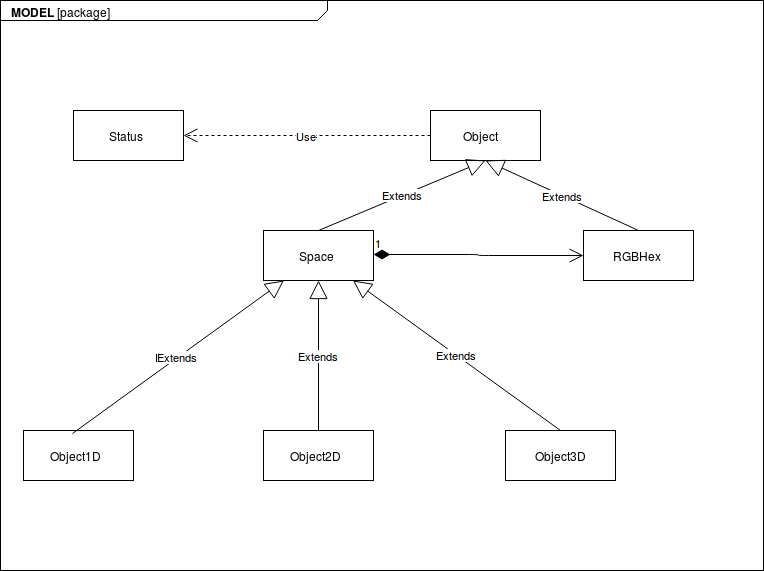
\includegraphics[scale=0.30]{Gerarchia.png}
   \caption{Gerarchia della parte Logica}
\end{figure}


\end{frame}

%------------------------------------------------

\begin{frame}
\frametitle{Classi Model}
\begin{itemize}
\item \textbf{Object} rappresenta una classe da cui deriva tutta la gerarchia, cosichè quando la \textit{BusinessLogic} andrà a fare operazioni sugli Object inseriti, a run time, eseguirà le operazioni esatte ed a aggiornerà lo \textit{Status} in modo adatto in base al tipo dinamico dell'Object selezionato.
\item \textbf{Space} classe Astratta rappresentante un Oggetto dimensionale avente un colore e una definizione di stampa (dpi), da cui poi ereditano \textit{Object1D}, \textit{Object2D} e \textit{Object3D}.
\item \textbf{Object1D} classe concreta che estende Space, possiede una lunghezza che determina se lo spazio dimensionale corrisponde a un punto unidimensionale (length=1) oppure un segmento.
\item \textbf{Object2D} classe concreta che estende Space, possiede una lunghezza e una altezza e rappresenta un sottoinsieme del piano cartesiano (oggetto bidimensionale).
\item \textbf{Object3D} classe concreta che estende Space, possiede una lunghezza, una altezza e una profondità e rappresenta un ogetto tridimensionale. 



\end{itemize}

\end{frame}

%------------------------------------------------

\begin{frame}
\frametitle{Classi Model}
\begin{itemize}
\item \textbf{RGBHex} classe concreta che deriva da Object, rappresenta un Colore RGB, costruibile tramite stringa (colore essadecimale), valori interi R G B.
Questa classe copre semplicemente il ruolo di colorare \textit{Object} e potenzialmente anche di interagire tramite operazioni su soli oggetti \textit{RGBHex}.

\item \textbf{Status} è una classe che svolge il ruolo di trasportatore; la classe Status è intrinseca in ogni classe derivante da Object, in quanto essa va ridefinita in base ai campi dati di quella classe. 

\item \textbf{BusinessLogic} è la classe che racchiude tutta la logica, tramite la funzione esegui che verrà richiamata dalla GUI con l'operatore "=" a run-time verrà scelto l'operazione adeguata ai tipi, inoltre fa da tramite con la GUI per tutto ciò che concerne la parte di Model.
\item \textbf{Exceptions} è la classe che contiene le classi di eccezioni che possono essere sollevate.
\end{itemize}
\end{frame}

%------------------------------------------------
\section{GUI}
%------------------------------------------------

\begin{frame}
\frametitle{GUI}
La GUI (Graphical User Interface) è strutturata:
\begin{enumerate}
\item MainWindow, da cui parte la creazione della BusinessLogic che a cascata verrà passata a tutti i sotto oggetti che comporranno il QGridLayout generale della calcolatrice, dopodichè viene costruito \textit{Contenitore}, che rappresenta, a tutti gli effetti, il layout generale di \textit{Space kalc}.

\item Contenitore, è la classe che crea effettivamente gli oggetti che permetterano la creazione di Object (tramite CreateObject), la selezione degli Object su cui si vuole fare operazioni (tramite Table) e infine la parte di calcolo (Calculate) che consentirà dopo aver inserito due Object tramite i QpushButton "add here", di selezionare un operatore e fare i dovuti calcoli.
\end{enumerate}
\end{frame}

%------------------------------------------------
\subsection{How to use} 
\begin{frame}
\frametitle{How to use GUI}
Più in dettaglio vediamo le 3 componenti di Contenitore:

   \FloatBarrier
   \begin{figure}[ht]
   \centering
   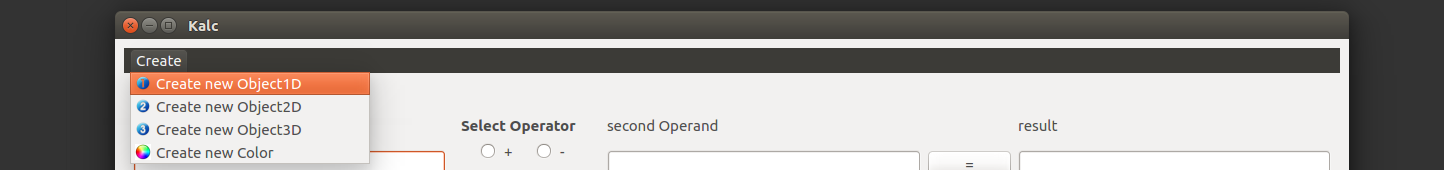
\includegraphics[scale=0.20]{Creazione.png}
   \caption{Create Object}
\end{figure}
Questa zona si trova nella parte superiore della calcolatrice dentro un QMenuBar, e attraverso Create (QMenu) si apre un menu a tendina (formato da QAction) che attraveso la pressione di quest'ultimi, vengono richiamati i costruttori di Oggetti e mostrati in una Finestra che si sovrapporrà a MainWindow.


   \FloatBarrier
   \begin{figure}[ht]
   \centering
   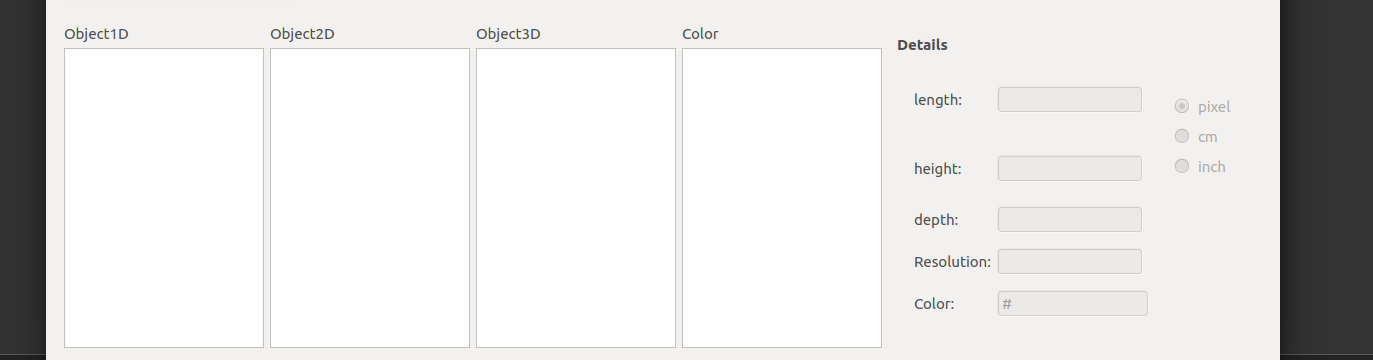
\includegraphics[scale=0.10]{Selezione.png}
   \caption{Selection Object}
\end{figure}


\end{frame}

%------------------------------------------------

\begin{frame} %[fragile] % Need to use the fragile option when verbatim is used in the slide
\frametitle{How to use GUI}
Una volta Creati gli Object, verranno inseriti all'interno degli appositi QListWidget (tramite iterazioni sui vector corrispondenti, fatti nella BusinessLogic che è stata precedentemente modificata con la creazione); questi Oggetti sono indicati da un indice e una volta selezionato un Object viene fatto vedere nella sezione \textit{Details} i rispettivi dettagli, inoltre è possibile vedere la corrispondente lunghezza in cm o inch.

   \FloatBarrier
   \begin{figure}[ht]
   \centering
   
\includegraphics[scale=0.10]{Calcolo.png}
   \caption{Calculate Object}
\end{figure}

Una volta selezionato un Object da un QListWidget è possibile aggiungerlo tramite uno dei QpushButton "add here", una volta aggiunti due Object, sarà possibile cliccare su un "QRadioButton" per selezionare l'operazione e avviare execute tramite il pulsante "=", se l'operazione sarà possibile tra i due tipi di Object verrà fatto vedere il risultato, altrimenti apparira un "QMessageBox" rappresentante il tipo di errore.



\end{frame}

%------------------------------------------------
\section{Caratteristiche kalc}
\begin{frame}
\frametitle{Caratteristiche}
\begin{itemize}
\item Polimorfismo è intrinseco nel Progetto
\begin{itemize}
\item operatori virtuali puri in Space, a run time verranno chiamati quelli ridefiniti nelle classi concrete.
\item getStatus funzione virtuale ridefinita in tutte le classi, a run time verrà aggiornato in base al tipo dinamico dell'Object su cui è stata invocata la funzione.
\item Unico modo in cui faccio \textit{RTTI} è tramite cast dinamico.

%Unico modo in cui faccio \textit{RTTI} è tramite "dynamic_cast".
\end{itemize}

\item Gli errori sono gestiti in due modi:
\begin{itemize}
\item per la parte Logica è stata creata un classe di eccezioni che vengono sollevate qual'ora le operazioni di 2 Object, invocate tramite execute(), non fossero possibili, inoltre sono stati fatti controlli preventivi per prevenire chiamate incomplete.
\item per la parte Grafica sono stati inseriti controlli preventivi, e qual'ora la correttezza dell'inserimento dei dati o l'operazione selezionata non fossero possibili, verrà visualizzato un QMessageBox all'interno del quale sarà descritto il tipo di errore. 

\end{itemize}

\end{itemize}
%\begin{figure}
%\includegraphics[width=0.8\linewidth]{test}
%\end{figure}
\end{frame}

%------------------------------------------------

\begin{frame}
\frametitle{Caratteristiche}
\begin{itemize}
\item La gestione della memoria è minoritaria in questo caso, poichè l'applicazione non fa uso pesante della memoria, l'unica cosa che viene allocata e modificata è la BusinessLogic nella GUI, ma quest'ultima non viene ricreata, ma viene passata attraverso tutte le varie componenti e modificata.
Mentre la Table che tiene visibili e aggiornati gli Object presenti nella BusinessLogic, viene ogni volta distrutta e ricreata.

\item \textit{Design Pattern} utilizzato è MVVM (Model View ViewModel) Questo pattern propone un ruolo più attivo della View rispetto a MVC: la View è in grado di gestire eventi, eseguire operazioni ed effettuare il data-binding. In questo contesto, quindi, alcune delle funzionalità del Controller vengono inglobate nella View, la quale si appoggia su un’estensione del Model.

\item Le ore rendicontate per lo svolgimento del Progetto sono pari a \textbf{50}, suddivise tra analisi dei Requisiti, decisioni progettuali, codifica, stesura relazione, trascrizione in Java, verifica e accettazione complessiva.
\end{itemize}
\end{frame}

%------------------------------------------------


%----------------------------------------------------------------------------------------

\end{document} 
